\hypertarget{ch2}{%
\chapter{Physiographic Controls on midwinter snowpack metrics in Sierra Nevada, CA}\label{ch2}}

%==============================================================================
%==============================================================================
%==============================================================================

\hypertarget{ch2-abstract}{\section{Abstract}\label{ch2-abstract}}

abstract

%==============================================================================
%==============================================================================
%==============================================================================
\hypertarget{ch2-intro}{\section{Introduction}\label{ch2-intro}}


Water resource management plans in the western US (WUS) are formulated around the assumption that the timing and magnitude of spring snowmelt is stable within the bounds of the interannual variability \citep{livnehDroughtLessPredictable2020}. Climate warming is affecting the stationarity of different processes in the hydrologic cycle all over the world \citep{millyStationarityDeadWhither2008}. In WUS, this means more cold season precipitation falling as rain, and warmer winter temperatures causing midseason melt.


-	On cloudy days, there’s little difference in CS insolation between aspect (cite). 


- hydroclimatic changes are driving increases in fire frequency and intensity \citep{abatzoglouImpactAnthropogenicClimate2016}, air temperatures (Hamlet \& Lettenmaier, 2007), midwinter dry spells \citep{hatchettMidwinterDrySpells2023}, could significantly impact society (cite). 

 
Warming temperatures have affected both the accumulation (cite) and ablation (cite) of mountain snowpack, which in turn. The Sierra Nevada is especially susceptible to these changes because its location is in the midlatitudes, where many of the catchments are low to mid-altitude basins, and small increases in temperature could push temperatures above 0 °C ore frequently \cite{gergelEffectsClimateChange2017}. These warming temperatures will affect both precipitation phase partitioning from snow to rain \citep{knowlesTrendsSnowfallRainfall2006}, which will decrease both snowfall amounts and snowpack cold content \citep{harpoldChangesSnowpackAccumulation2012a}. \cite{nolinMappingRiskSnow2006} characterized this type of snow as "at-risk" or snow with the highest potential of being affected by warming temperatures. 

Past studies have leveraged in situ data and models to evaluate snowpack metric trends \citep{clowChangesTimingSnowmelt2010,haleRecentDecreasesSnow2023,harpoldChangesSnowpackAccumulation2012a, moteDECLININGMOUNTAINSNOWPACK2005, moteDramaticDeclinesSnowpack2018, musselmanWinterMeltTrends2021} and the physical mechanisms that govern snowpack snow accumulation and ablation \citep{harpoldHumidityDeterminesSnowpack2018}. Snow pillows cover less than 1 \% of the land area and are limited to mainly mid-elevation flat forest cuts \citep{guan20102011Snow2013}, and macroscale hydrologic models like Variable Infiltration Capacity (VIC) \citep{liangSimpleHydrologicallyBased1994} have resolutions on the scale of kilometers — neither are well-suited for understanding snowpack patterns in complex topography. These physiographic factors impact the local energy balance dynamics, which govern the accumulation and ablation of the snowpack. \cite{musselmanWinterMeltTrends2021} notes the importance of understanding physiographic relationships of snowpack metrics and climatology; therefore, allowing a grasp of how these areas will change (***rework***). \cite{pomeroyVariationSurfaceEnergetics2003} used in situ meteorologic instrumentation setup slope normal, instead of the traditional gravimetric orientation, and found marked differences in incoming shortwave radiation (SW$_{in}$) and ablation rates on south and north facing slopes (**rework**).
-paragraph on snowpack metrics: what are they, why are they important, cite (Nolin et al., 2021)

Previous studies characterized snowpack metrics with respect to physiography. \cite{trujilloSnowpackRegimesWestern2014} used SNOTEL data over the WUS to quantify specific snowpack regimes. \citep{tennantRegionalSensitivitiesSeasonal2017, molotchEcohydrologicalControlsSnowmelt2009} 

 - What is our, “In this study we…” statement?? \

To better understand how snowpack will react to warming temperatures, we must quantify the physiographic controls on hydrologically important snowpack metrics. Here, we utilize the Sierra Nevada Snow Reanalysis (SNSR), a 90 m spatiotemporally continuous SWE data set from 1985–2016 (32 years), for a comparison of how snowpack metrics change with physiography, specifically aspect and elevation. We analyze three common snowpack metrics: max SWE (MSWE), day of max SWE (DOM), fraction of snow ablation before 1 April (FM) (Musselman et al., 2021), and amount of snow ablation (MWA). We then compare these metrics against annual temperature and a clear sky shortwave radiation (herein SWin) and perform a Spearman’s Rho (SR) (Yue et al., 2002).

NEW THOUGHTS
The magnitude of insolation absorbed at the snow surface is a function of various physical factors. Aspect is a first-order control and the directness and total magnitude of insolation received in a given area. Thus, impacts the snow albedo, with south facing slopes having recieve more insolation a lower albedo***. The type and density of vegetation overlaying the snow surface can significantly impact the amount of insolation received at the snow surface (cite roth) canopy, with dense conifers shading nearly all incoming radiation. The energy input and hydrologic variabilty between aspects inturn effect vegetation (webb et al. 2023), soil moist  and  These differences vary temporally with seasons as the solar declines and inclines, the with the winter months having the most marked differences and radiative inputs.


Canopy cover variations, from either disturbance or management, was not specifically addressed in the SNSR modeling framework.  



ANNE NOTES
- it is key to disaggregate by physiographic parameters which serve as key controls on snowpack energy balance, thus we focus the effects slope and aspect on key snow metrics. \

-info on blowing snow and redistribution
- While detection of monotonic trend is useful for understanding that a given metric is changing, understanding the physical mechanism (i.e., temperature, SW, LW) driving that change illuminates 
-	How does elevation impact SWE, snowfall? How does landscape? \

-	What about slope and aspect? \citep{dozierRevisitingTopographicHorizons2022, dozierApproachEnergyBalance1979} \

-	Why is FM greater lower elevations: rain-snow partitioning/storm temperature \citep{huWidespreadWarmingTrends2020} warmer (temps), \

-	From Musselman: “To explain the elevation-dependent trends and assess whether the observed dynamics are captured in models are beyond the scope of this paper. More generally, an increased understanding of the climatological and physiographical dependencies of snowpack sensitivities to anthropogenic climate warming is needed.” \

-	(A. A. Harpold \& Brooks, 2018) “The observation that seasonal snow cover in the western United States exists across a mean winter temperature range of greater than 12 °C, including multiple locations with mean winter temperatures greater than 0 °C (Fig. 4), highlights the importance of other energy fluxes in controlling snowpack response to climate change.” \

-	While many past studies have leveraged in situ data to evaluate both trends and the physical mechanisms that govern snowpack accumulation and ablation, none have addressed how physiographic variables (e.g. slope and aspect) impact these due to data deficiencies. \

 

%==============================================================================
%==============================================================================
%==============================================================================
\hypertarget{ch2-sa}{\section{Study Area}\label{ch2-sa}}

We choose three distinct river basins to analyze: the Yuba, Upper San Joaquin (USJ), and the Kern. These basins are described below.

- mean temp, cc, how many elevation zones, slope, aspect, ect,

fraction of area of NF and SF per basin

%f1
\begin{figure*}[t]
\centering
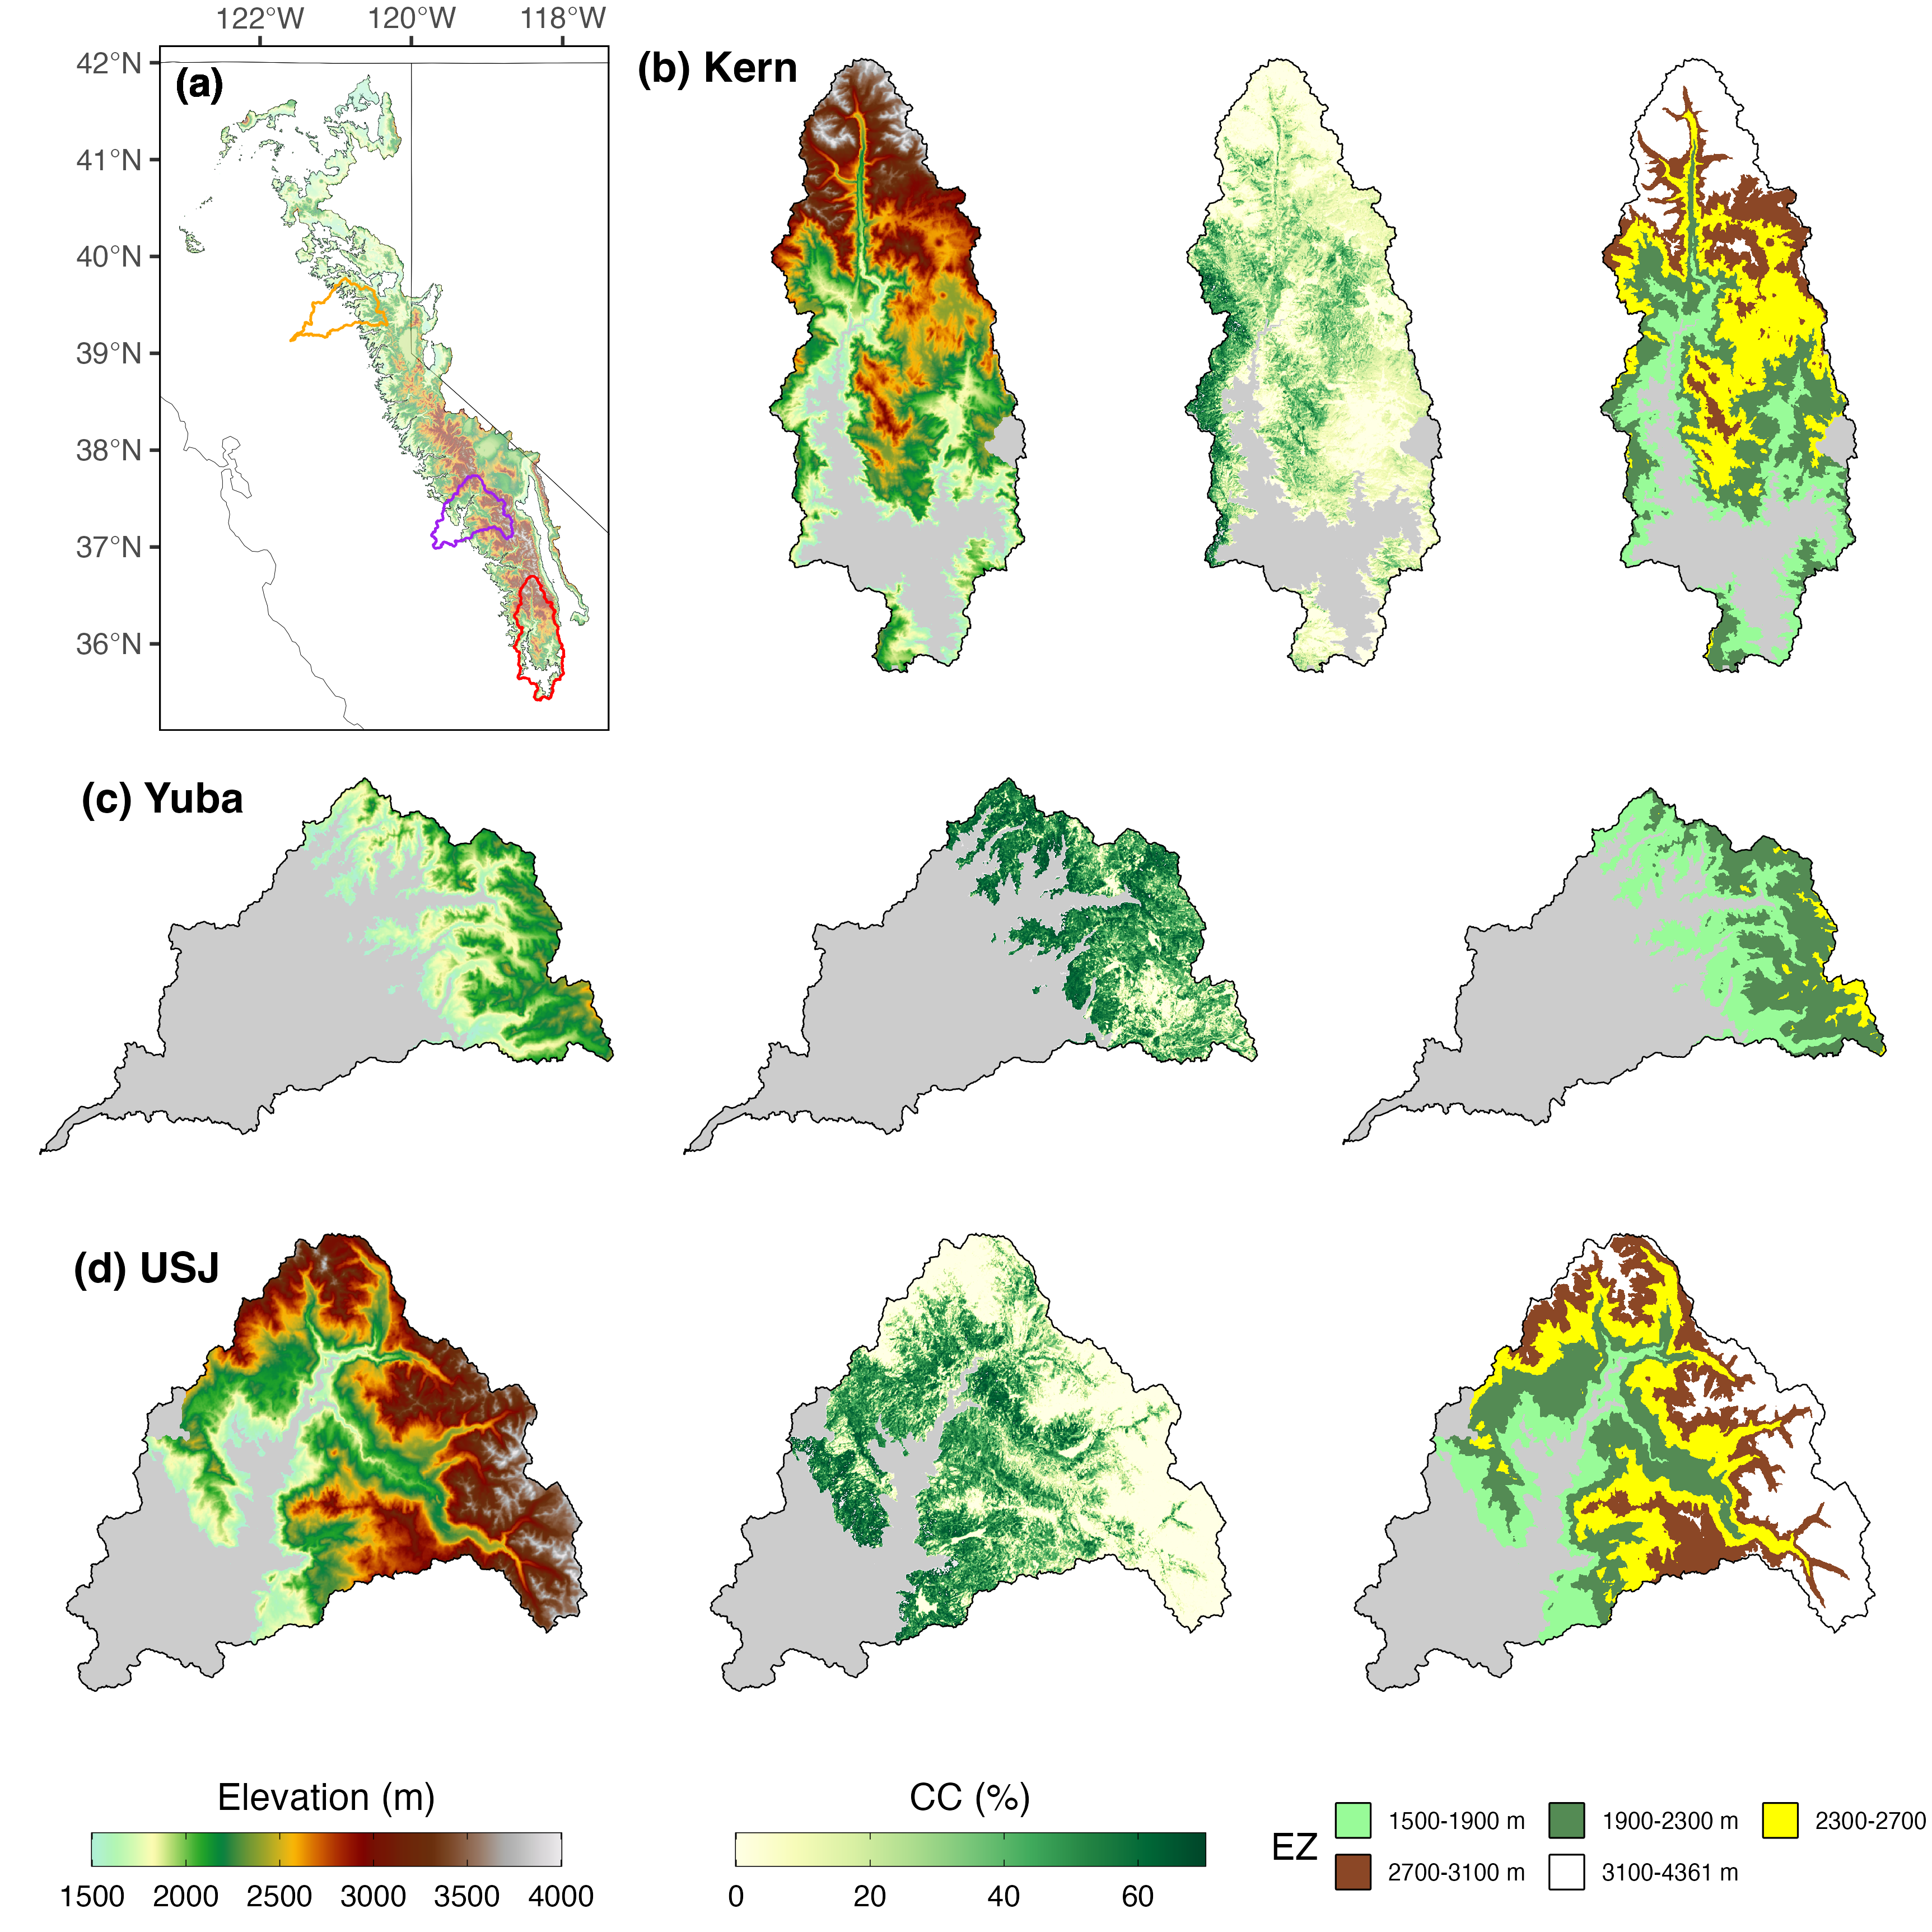
\includegraphics[width=14cm]{figures/ch2_figs/kuy_study_area_v2.png}
\caption{\textbf{(a)} The full extent of the SNSR study domain with Yuba (orange), USJ (purple), and Kern (red) basins shown. From left to right for the \textbf{(b)}~Kern, \textbf{(c)}~Yuba, \textbf{(d)}~USJ: elevation, canopy cover (\%), and elevation zones (EZs).}
\label{kuy_study_area}
\end{figure*}
%==============================================================================
\hypertarget{ch2-sa-1}{\subsection{Yuba}\label{ch2-sa-1}}


%==============================================================================
\hypertarget{ch2-sa-2}{\subsection{USJ}\label{ch2-sa-2}}


%==============================================================================
\hypertarget{ch2-sa-3}{\subsection{Kern}\label{ch2-sa-3}}


%==============================================================================
%==============================================================================
%==============================================================================
\hypertarget{ch2-do-1}{\section{Data Overview}\label{ch2-do-1}}

In this section we describe the data products used in this study.

%==============================================================================
\hypertarget{ch2-do-2}{\subsubsection{SNSR}\label{ch2-do-2}}


The Sierra Nevada SWE Reanalysis (SNSR) \citep{margulisLandsatEraSierraNevada2016} is a 90~m gridded daily SWE product for California Sierra Nevada from water year (WY) 1985--2016. These data were created using a Bayesian particle batch smoother data assimilation (DA) technique to retroactively assimilate Landsat fractional snow-covered area (fSCA) with downscaled National Land Data Assimilation System (NLDAS) meteorologic forcing. The MSWE estimates were validated with over 9000 years of snow pillow and snow course data. Detailed information on the development and implementation of this methodology can be found in a series of past publications: \cite{durandBayesianApproachSnow2008, girottoExaminingSpatialTemporal2014, girottoProbabilisticSWEReanalysis2014, margulisParticleBatchSmoother2015}. A recent analysis from \citep{yangIntercomparisonSnowWater2023} evaluated the uncertainty of various SWE products using ASO lidar data. They found that the SNSR performed the best according to various error metrics, making it a well-suited dataset for our analysis.

\hypertarget{ch2-do-2}{\subsubsection{SNOTEL data}\label{ch2-do-2}}

We used snow pillow data form 29....

\hypertarget{ch2-do-2}{\subsubsection{gridMET Data}\label{ch2-do-2}}

We used 4~km meteorological data from gridMET \citep{abatzoglouDevelopmentGriddedSurface2013} to calculate annual (1985--2016) cold season values from October 1 to March 31 (ONDJFM) for four meteorologic variables: mean temperature(T\textsubscript{mean}), relative humidity (RH\textsubscript{mean}), incoming solar radiation (insolation), absolute humidity (AH). Daily ONDJFM where averaged to create the annual metrics. These data were bilinearly downscaled to the 90 m SNSR resolution.Since gridMET does not include a T\textsubscript{mean} or RH\textsubscript{mean} value, only the daily maximum and minimum, these values were averaged to create the two mean variables. Insolation from gridMET is estimated with respect to a planar surface and not topographically corrected. AH in g~cm$^{-3}$ was calculated using T\textsubscript{mean}, RH\textsubscript{mean}, and a function based off the ideal gas law:

\begin{equation}
\text{AH} = \frac{{6.112 \times e^{\left(\frac{{17.67 \times \text{T}\textsubscript{mean}}}{{\text{T}\textsubscript{mean} + 243.5}} \right)} \times \text{RH}\textsubscript{mean} \times 2.1674}} {{273.15 + \text{T}\textsubscript{mean}}}
\label{eq:ah}
\end{equation}


%==============================================================================
\hypertarget{ch2-do-2}{\subsubsection{Clear sky insolation}\label{ch2-do-2}}


We estimated 90~m spatially distributed mean ONDJFM clear sky incoming solar radiation (CS insolation) using the R package “insol”, which is based on the Bird model \citep{birdReviewEvaluationImprovement1981}. The model uses the SNSR 90 m DEM as input and accounts for slope, aspect, differential shading, day of year, solar zenith angle, air temperature, elevation, and relative humidity. We held these values constant, with information on the specific model parametrization included in the supplement***. To calculate CS insolation the daily values were averaged in the same fashion as the gridMET data. This produced a single estimate not a time series like gridMET data.


%==============================================================================
%==============================================================================
%==============================================================================
\hypertarget{ch2-methods}{\section{Methods}\label{ch2-methods}}
\hypertarget{ch2-methods-1}{\subsection{Snow metric creation and validation}\label{ch2-methods-1}}

\begin{figure*}[t]
\centering
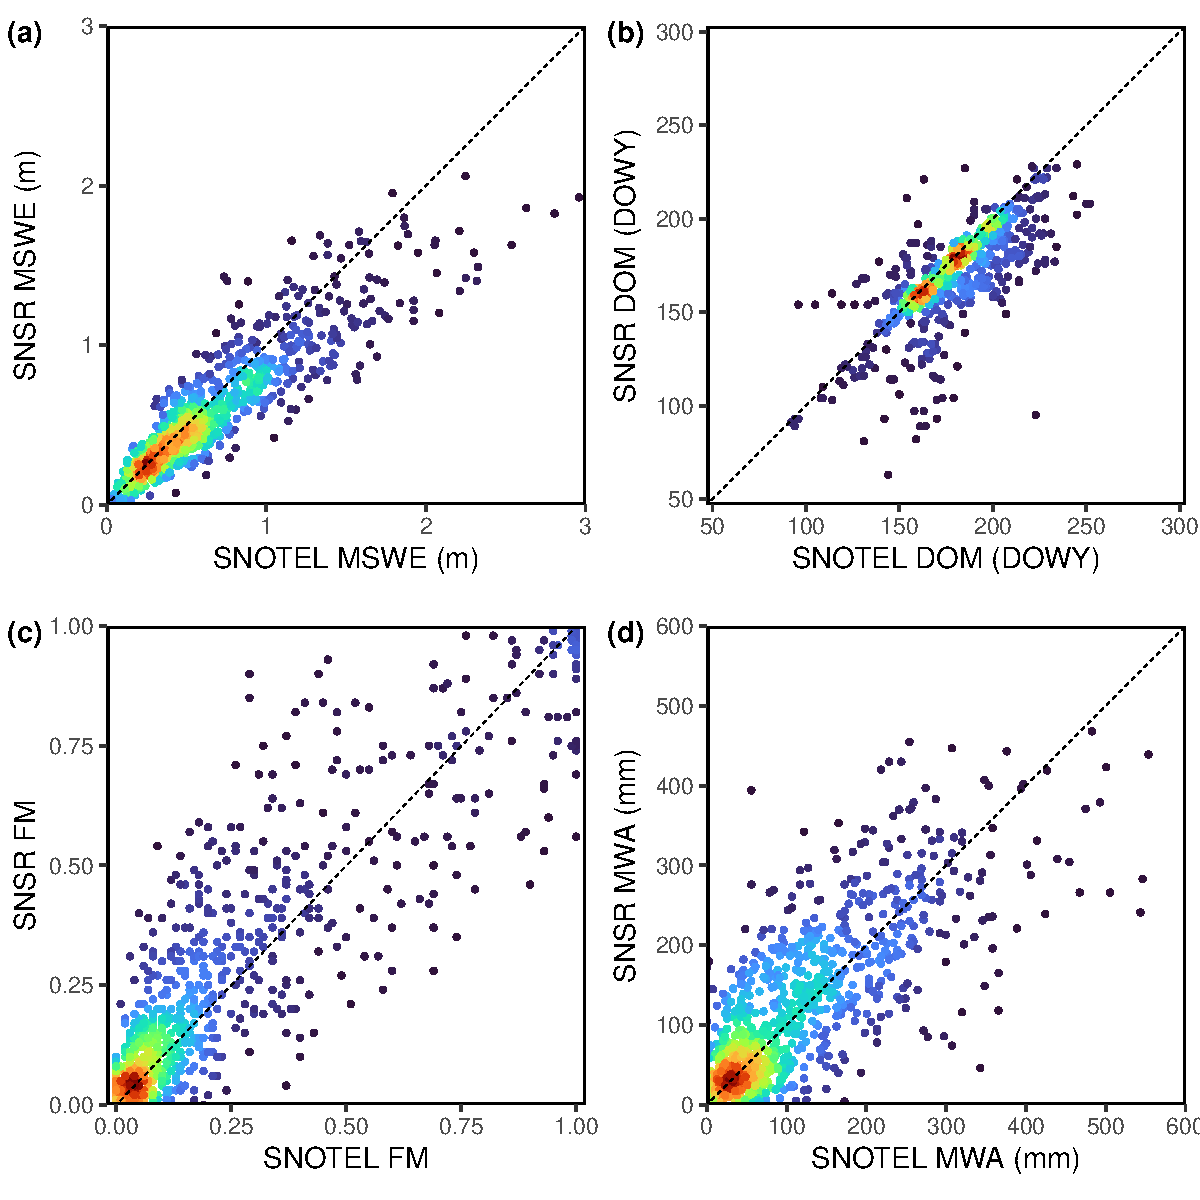
\includegraphics[width=10cm]{figures/ch2_figs/snsr_snotel_metric_compare_new_v1.pdf}
\caption{Density plots comparing SNSR and SNOTEL \textbf{(a)} MSWE, \textbf{(b)} DOM, \textbf{(c)} FM days, \textbf{(d)} MWA for 29 SNOTEL stations from WY 1985--2016 (n $\approx$ 840).}
\label{kuy_study_area}
\end{figure*}

Using the SNSR, we generated four pixel-wise snowpack metrics: MSWE, DOM, FM, and MWA. MSWE is defined as the maximum amount (mm) of SWE in a given pixel for WY, while DOM is the last day of water year which the pixel has the amount. FM is the fraction of ablation (melt, wind transport, sublimation) that occurs before April 1st, while MWA is the amount of SWE lost in (mm). Reporting both FM and MWA allows for a more complete understanding of midwinter melt dynamics, as gives two different values to melt across the landscape (***rework***).

We focused on our analysis on the seasonal snow zone, or areas that receive snow that majority of years. To do this, an annual accumulation threshold of 26~mm ($\sim$1~in) was of SWE for a given pixel to be considered. Then, within the 32-year time series, a pixel must meet this condition at least 27 of the 32 years. ***See Appendix 1 for figures showing the full SNSR study area***. 

SNSR values were selected by the specific pixel in which the station fell. These metrics were then validated against 29 SNOTEL stations totaling $\sim$840 station years (Figure \ref{kuy_study_area}). Two correlation coefficients (R and R$^{2}$), root-mean-square error (RMSE), mean absolute error (MAE), mean error (ME), and percent bias (PB) are in Table \ref{tab:snow_metrics_val_table}.

\begin{table}[htbp]
  \centering
  \caption{Error statistics (RMSE, MAE, ME, and PB) and correlation coefficients for (R and R$^{2}$) for the MSWE, DOM, and FM compared to 29 SNOTEL stations from WY 1985–-2016 (n $\approx$ 840). The in situ data are compared against the single SNSR pixel in which the station falls within.}
  \label{tab:snow_metrics_val_table}
  \begin{tabular}{lllllll}
    \toprule
    Snow Metric & R & R$^{2}$ & RMSE & MAE & ME & PB (\%) \\
    \midrule
    Max SWE (m) & 0.9 & 0.81 & 0.22 & 0.15 & $-$0.08 & $-$11.6 \\
    Max SWE (DOWY) & 0.75 & 0.56 & 18.95 & 11.59 & $-$8.05 & $-$4.5 \\
    FM & 0.88 & 0.77 & 0.14 & 0.09 & 0.03 & 12.5 \\
    MWA (mm) & 0.75 & 0.56 & 71.78 & 52.44 & 9.06 & 7.4 \\
    \bottomrule
  \end{tabular}
\end{table}

\hypertarget{ch2-methods-2}{\subsection{Spearman correlations}\label{ch2-methods-2}}

Spearman's Rho, a non-parametric measure of statistical dependence between variables, was computed to assess the relationship between FM and the three meteorological variables across the EZs and three study basins. The goal of this analysis was to characterize the snow metric sensitivity to the meteorologic data.

%==============================================================================
%==============================================================================
%==============================================================================
\hypertarget{ch2-results}{\section{Results}\label{ch2-results}}
\hypertarget{ch2-results-1}{\subsection{Snow metric physiography}\label{ch2-results-1}}

The four snowpack metrics varied significantly with patterns emerging with respect to basin, elevation, and aspect. The mean values---split into north and south facing slopes and EZs---for the four snow metrics are displayed in Table \ref{tab:snow_metric_table} and the boxplots showing the distribution in Fig.\ref{fig:snow_boxplots}. We also report the physiographic distribution of the four meteorologic variables in Table \ref{tab:met_metric_table} and Fig. \ref{fig:met_boxplots}.

%f1
\begin{figure*}[t]
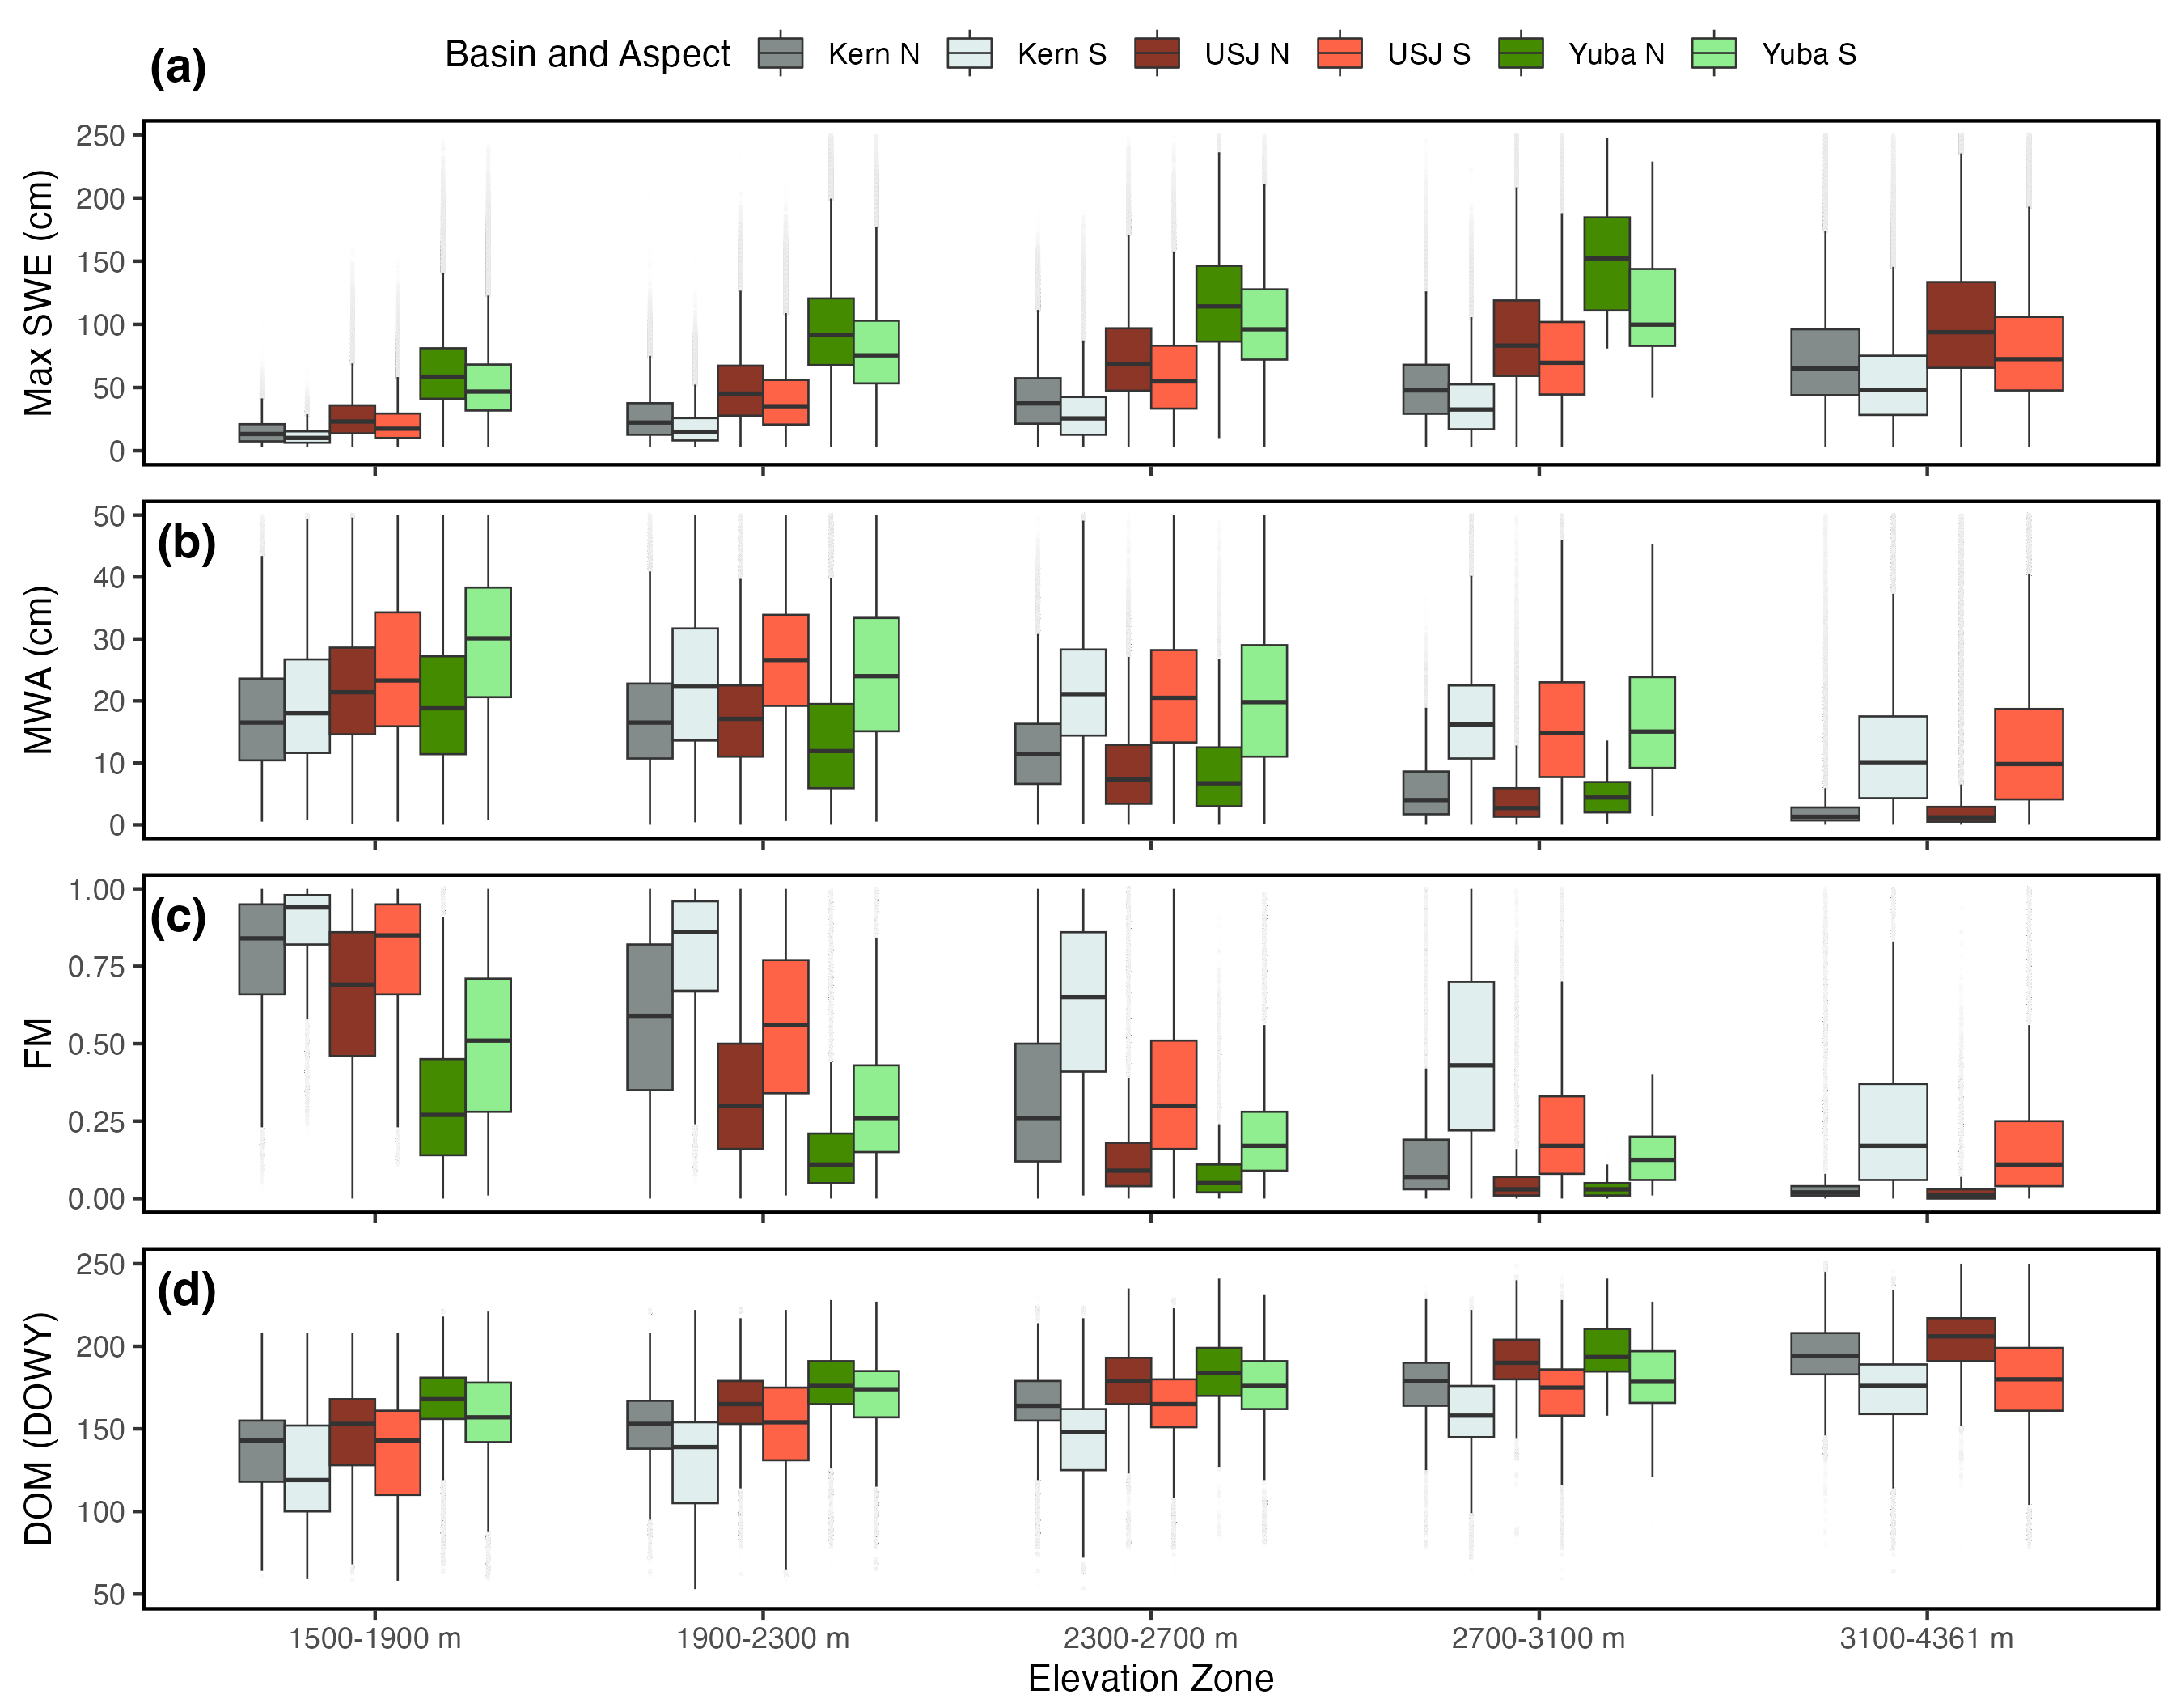
\includegraphics[width=\textwidth]{figures/ch2_figs/snow4_boxplot_v5.png}
\caption{Boxplots for \textbf{(a)} MSWE, \textbf{(b)} MWA, \textbf{(c)} FM, \textbf{(d)} DOM, for the 32-year study period. The data are grouped by the five EZs and colored the three basins: Kern (gray), USJ (orange), Yuba (green). The colors shading represents north facing (darker) and south facing (lighter) slopes for the respective basin.}
\label{fig:snow_boxplots}
\end{figure*}


For all of the snow metrics in all three basins, there are marked differences between the north and south facing slopes \ref{fig:snow_boxplots}. Overall the Kern, the southern most basin, has the greatest mean FM values (Fig. \ref{fig:snow_boxplots}a) for all elevation bands when compared to the Yuba and the USJ. Additionally, it had the highest mean FM percent difference between south and north facing slopes of 69.6~\%. Yet, shown in Fig. \ref{fig:met_boxplots} and Table \ref{tab:met_metric_table}, the Kern has either similar or colder T\textsubscript{mean} values (Fig. \ref{fig:met_boxplots}a) than the Yuba and the USJ. These differences can be explained by the insolation values in the Kern (Fig. \ref{fig:snow_boxplots}c) being greater by $\sim$15--25 $\mathrm{W~m}^{-2}$ across all EZs. Elevation trends are consistently observed across all three basins for each of the four metrics, although the magnitude of the differences varies incongruently among the basins. As expected, MSWE and DOM increase with elevation, while FM and MWA broadly decrease.

The two midwinter ablation metrics (FM and MWA) impact both MSWE and DOM for all basins and EZs. Across the three basins, south facing slopes reach DOM 16.1~d earlier, with the greatest mean difference of 25 d occuring in the USJ between 3100--4361~m.

For EZ4 (2700--3100~m) and EZ5 (3100--4361~m), the USJ and Kern showed particularly stark differences in both midwinter ablation metrics with respect to aspect. The mean FM and MWA values for the two basins in these elevation zones on north facing slopes were 0.07 and 39~mm, respectively. In contrast, south facing slopes had markedly higher values, with mean FM and MWA values of 0.29 and 151~mm. This means there is approximately 4 times more FM and MWA on south facing slopes at elevations above 3100~m. Furthermore, the T\textsubscript{mean} values are below 0$^{\circ}$ for these errors. This suggests insolation as a driving factor in midwinter ablation.


For the gridMET derived metrics (T\textsubscript{mean}, RH***, insolation) there are no significant difference between the north facing and south facing slopes (Figure \ref{fig:met_boxplots}.a--c). This makes sense considering griMET's 4~km spatial resolution, thus not capturing the topographic heterogeneity of the 90~m SNSR data. CS insolation shows vast differences in the amount insolation received by the two aspects. Across all basins and EZs, South facing slopes have a mean daily value of 234 $\mathrm{W~m}^{-2}$, while north facing's is 43 $\mathrm{W~m}^{-2}$. Since these are static clear sky estimates, the values say consistent across the three study basins and EZs.

Clear elevational and aspect patterns emerge. For the two ablation metrics (MWA and FM), we see stark differences, which are ampflied as elevation increases.


FM and MWA impact both MSWE and DOM


\begin{table}[htbp]
\centering
\caption{The mean values of the MWSE, DOM, FM, and FM for the three study basins. Each basin is split into north facing (NF) and south facing (SF) with the difference between the two also shown.}
\label{tab:snow_metric_table}
\tiny % Reduce font size to \small
\begin{tabular}{llrrrrrrrrrrrr}
\toprule
& & \multicolumn{3}{c}{MSWE (mm)} & \multicolumn{3}{c}{DOM (DOWY)} & \multicolumn{3}{c}{FM} & \multicolumn{3}{c}{MWA (mm)} \\
\midrule
Basin & EZ & NF & SF & Diff & NF & SF & Diff & NF & SF & Diff & NF & SF & Diff \\
\midrule
Kern & 1500--1900 m & 151 & 116 & -35 & 138 & 127 & -11 & 0.78 & 0.87 & 0.09 & 178 & 201 & 23 \\
Kern & 1900--2300 m & 269 & 191 & -78 & 149 & 133 & -16 & 0.58 & 0.79 & 0.21 & 171 & 238 & 67 \\
Kern & 2300--2700 m & 414 & 301 & -113 & 164 & 143 & -21 & 0.34 & 0.62 & 0.28 & 119 & 222 & 103 \\
Kern & 2700--3100 m & 518 & 375 & -143 & 178 & 156 & -22 & 0.15 & 0.47 & 0.32 & 56 & 177 & 121 \\
Kern & 3100--4361 m & 744 & 555 & -189 & 195 & 173 & -22 & 0.04 & 0.25 & 0.21 & 25 & 123 & 98 \\
USJ & 1500--1900 m & 267 & 219 & -48 & 146 & 136 & -10 & 0.65 & 0.78 & 0.13 & 218 & 262 & 44 \\
USJ & 1900--2300 m & 505 & 411 & -94 & 163 & 149 & -14 & 0.35 & 0.56 & 0.21 & 172 & 282 & 110 \\
USJ & 2300--2700 m & 745 & 614 & -131 & 178 & 162 & -16 & 0.14 & 0.35 & 0.21 & 87 & 221 & 134 \\
USJ & 2700--3100 m & 927 & 771 & -156 & 191 & 172 & -19 & 0.06 & 0.24 & 0.18 & 43 & 170 & 127 \\
USJ & 3100--4361 m & 1068 & 808 & -260 & 204 & 179 & -25 & 0.03 & 0.18 & 0.15 & 31 & 133 & 102 \\
Yuba & 1500--1900 m & 637 & 531 & -106 & 166 & 153 & -13 & 0.31 & 0.5 & 0.19 & 203 & 335 & 132 \\
Yuba & 1900--2300 m & 960 & 809 & -151 & 176 & 168 & -8 & 0.15 & 0.31 & 0.16 & 136 & 272 & 136 \\
Yuba & 2300--2700 m & 1210 & 1020 & -190 & 184 & 174 & -10 & 0.08 & 0.21 & 0.13 & 85 & 221 & 136 \\
Yuba & 2700--3100 m & 1660 & 1193 & -467 & 196 & 178 & -18 & 0.04 & 0.15 & 0.11 & 61 & 178 & 117 \\
\bottomrule
\end{tabular}
\end{table}

\hypertarget{ch2-results-2}{\subsection{met}\label{ch2-results-2}}

helllo

\begin{figure*}[t]
\centering
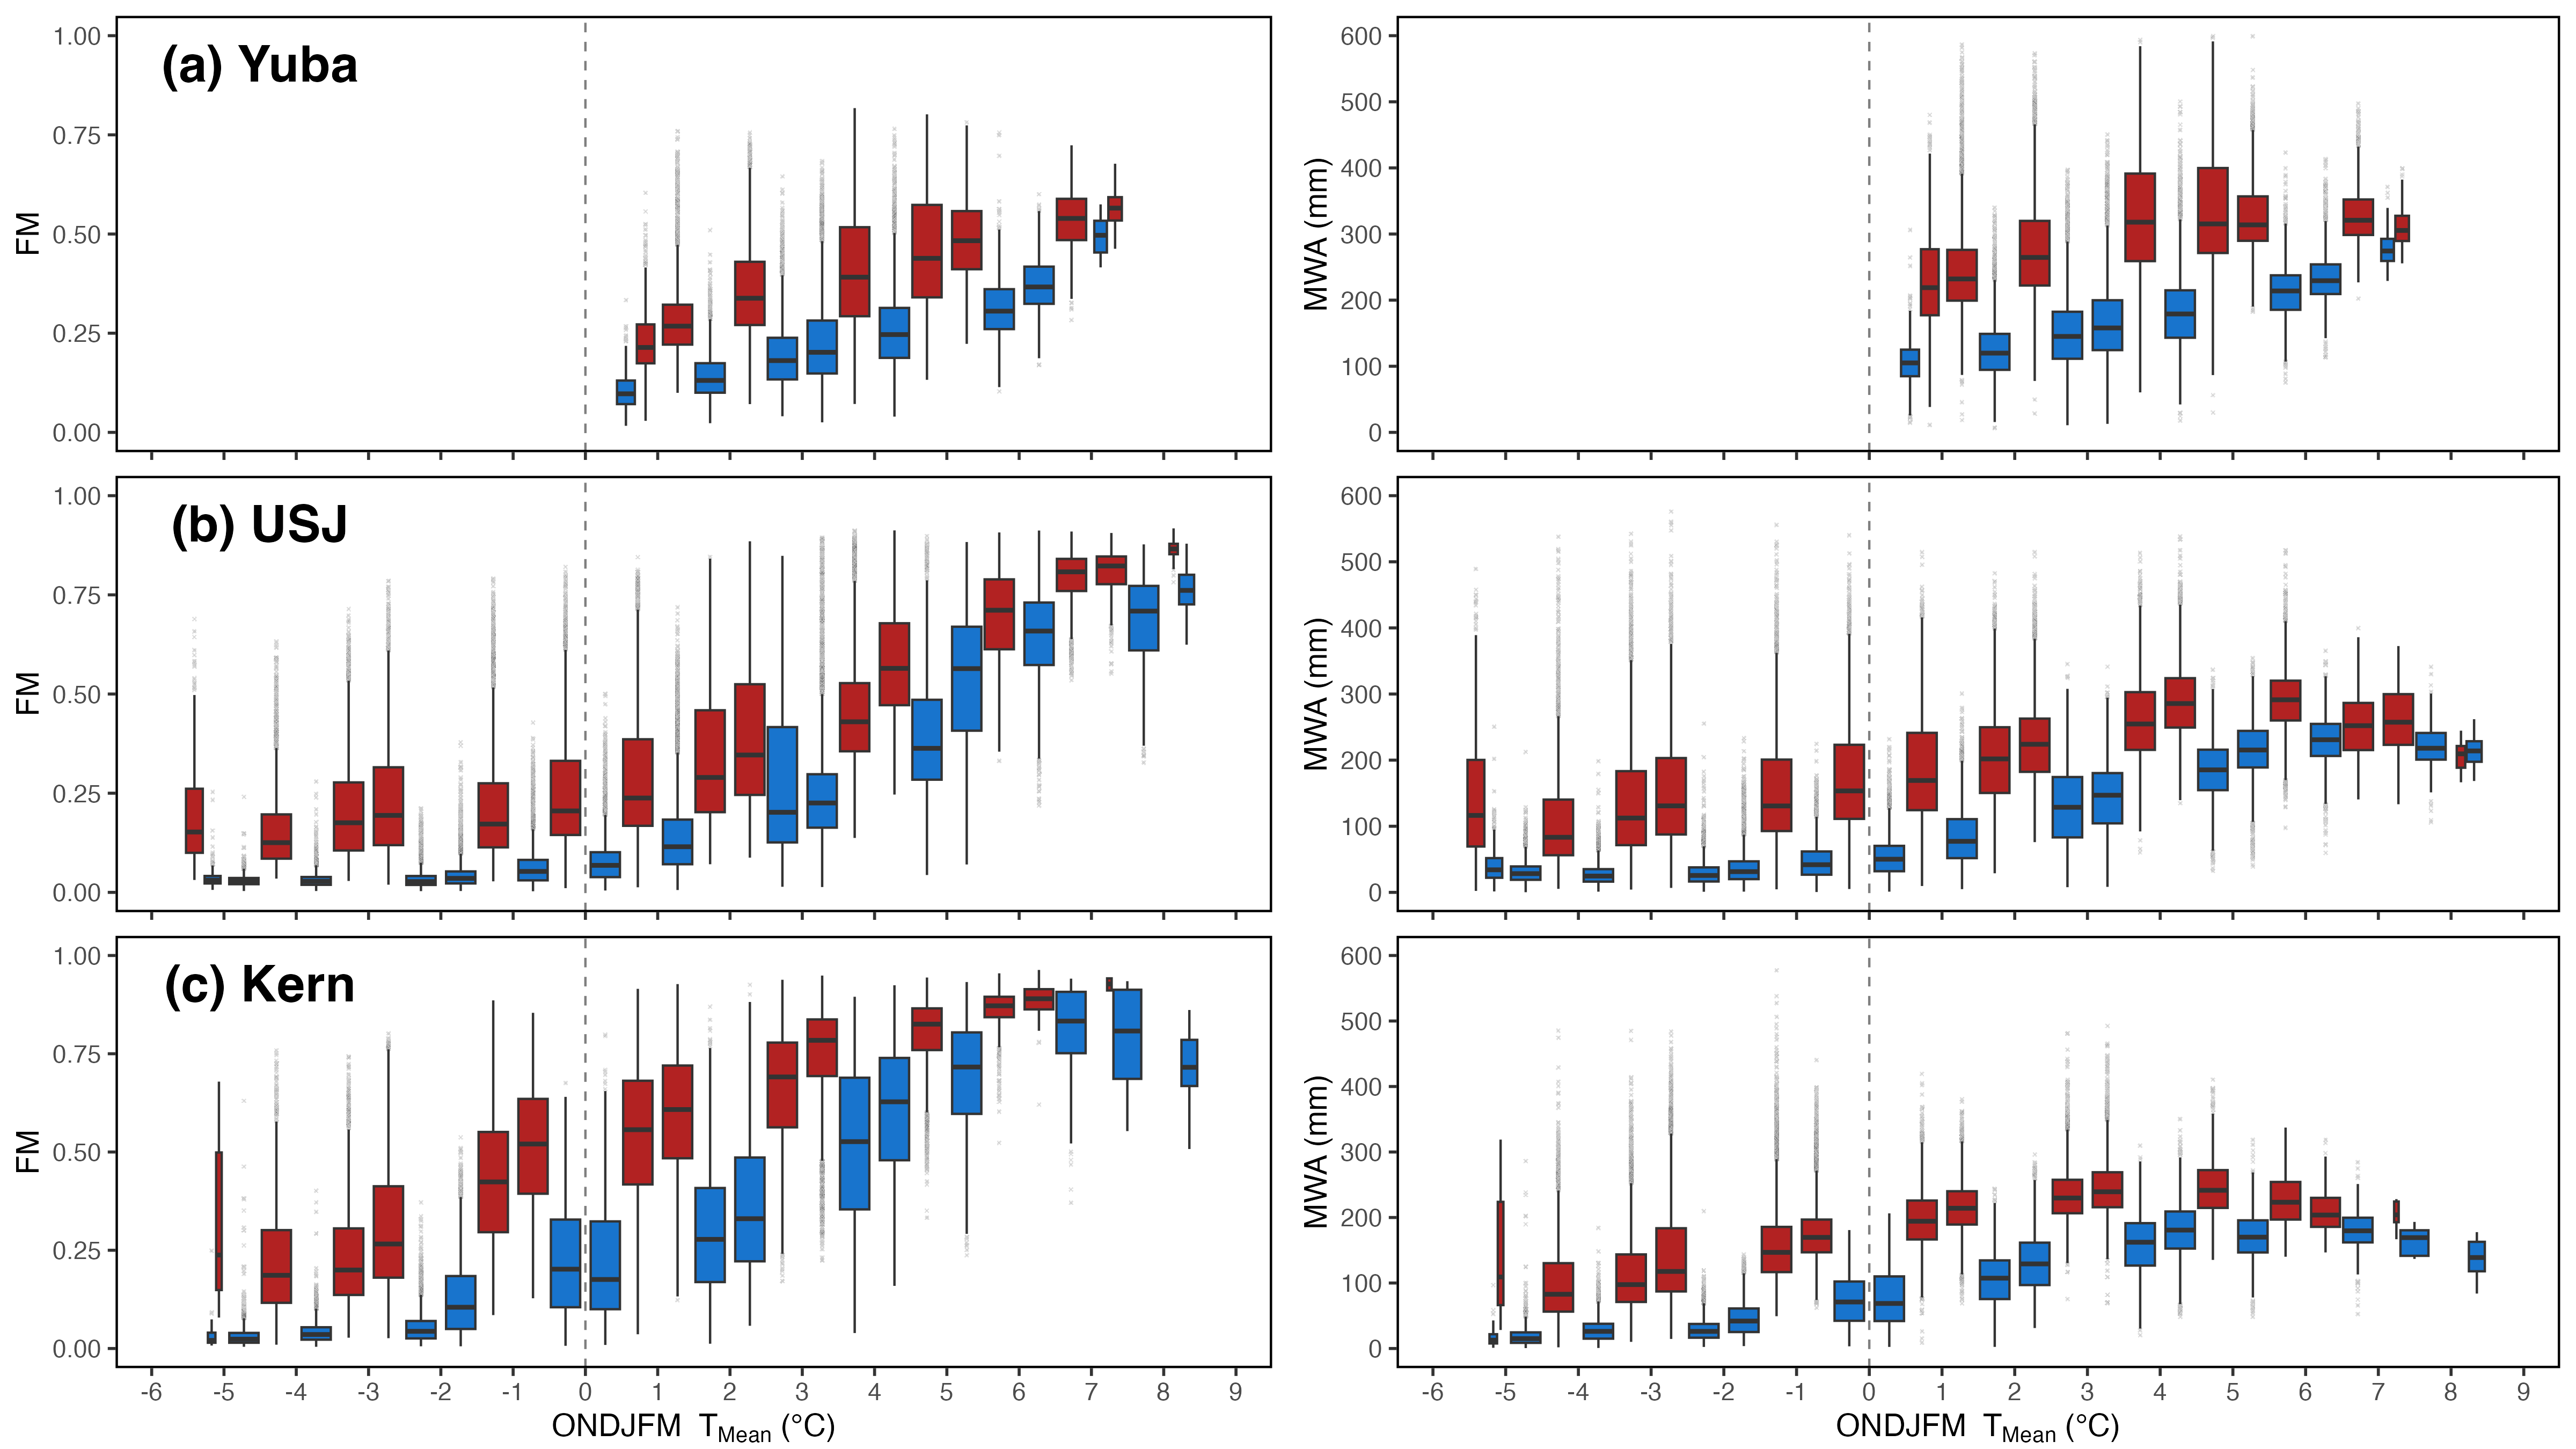
\includegraphics[width=\textwidth]{figures/ch2_figs/aspect_temp_mwa_fum_full_boxplots_v2.png}
\caption{Boxplots comparing FM (left) and MWA (right) on north facing (blue) and south facing (red) slopes for the \textbf{(a)} Yuba, \textbf{(b)} USJ, \textbf{(c)} Kern.}
\label{fig:aspec_mwa_fm_bp}
\end{figure*}

\begin{figure*}[h]
\centering
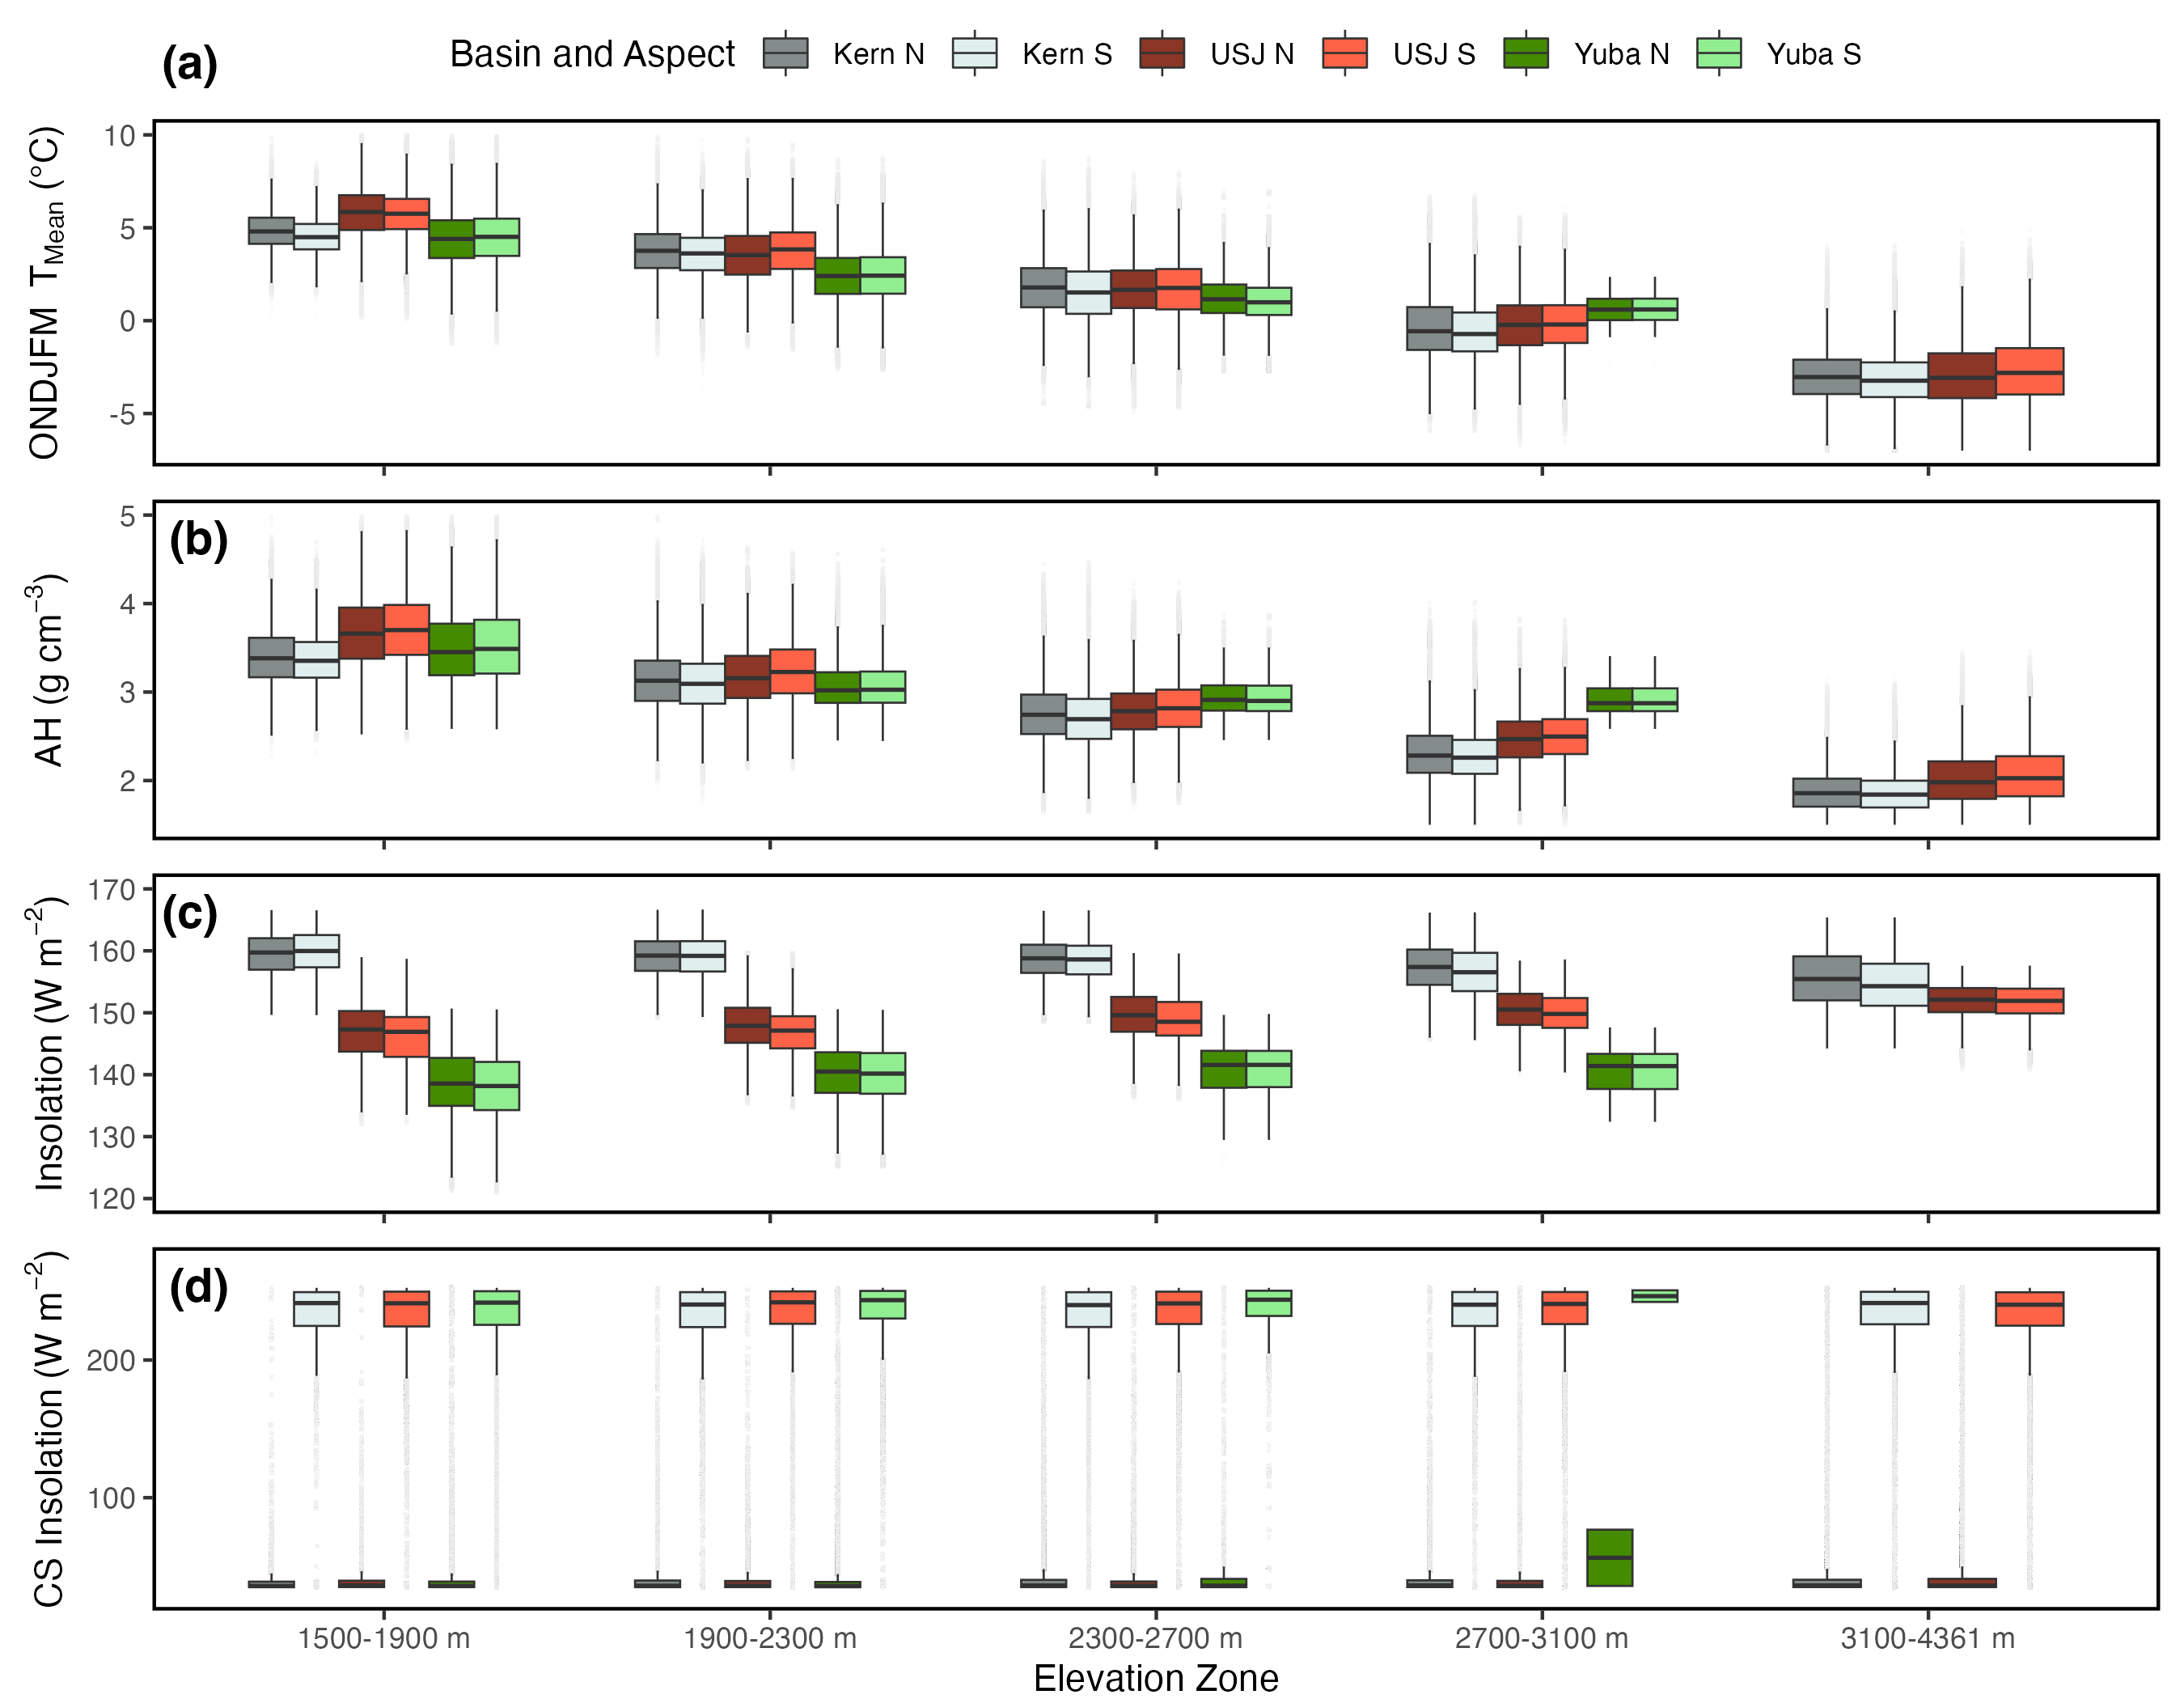
\includegraphics[width=\textwidth]{figures/ch2_figs/met4_boxplot_v4.png}
\caption{ Boxplots for \textbf{(a)} T\textsubscript{mean}, \textbf{(b)} AH, \textbf{(c)} insolation, and \textbf{(d)} CS insolation for the 32-year study period. The data are grouped by the five EZs and colored the three basins: Kern (gray), USJ (orange), Yuba (green). The colors shading represents north facing (darker) and south facing (lighter) slopes for the respective basin.}
\label{fig:met_boxplots}
\end{figure*}



\begin{table}[htbp]
\centering
\caption{The mean values of the T\textsubscript{mean}, AH, insolation, and CS insolation for the three study basins. Each basin is split into north facing (NF) and south facing (SF) with the difference between the two also shown.}
\label{tab:met_metric_table}
\tiny 
\begin{tabular}{llrrrrrrrrrrrr}
\toprule
& & \multicolumn{3}{c}{T\textsubscript{mean}} & \multicolumn{3}{c}{AH} & \multicolumn{3}{c}{Insolation} & \multicolumn{3}{c}{CS Insolation} \\
\midrule
Basin & EZ & NF & SF & Diff & NF & SF & Diff & NF & SF & Diff & NF & SF & Diff \\
\midrule
Kern & 1500-1900 m & 4.98 & 4.68 & -0.3 & 3.4 & 3.37 & -0.03 & 159 & 159 & 0 & 41 & 231 & 190 \\
Kern & 1900-2300 m & 3.86 & 3.68 & -0.18 & 3.14 & 3.1 & -0.04 & 159 & 158 & -1 & 41 & 232 & 191 \\
Kern & 2300-2700 m & 1.83 & 1.56 & -0.27 & 2.75 & 2.7 & -0.05 & 158 & 158 & 0 & 41 & 232 & 191 \\
Kern & 2700-3100 m & -0.39 & -0.55 & -0.16 & 2.31 & 2.28 & -0.03 & 157 & 156 & -1 & 41 & 233 & 192 \\
Kern & 3100-4361 m & -2.98 & -3.13 & -0.15 & 1.85 & 1.83 & -0.02 & 155 & 154 & -1 & 46 & 233 & 187 \\
USJ & 1500-1900 m & 5.83 & 5.78 & -0.05 & 3.67 & 3.7 & 0.03 & 147 & 146 & -1 & 40 & 232 & 192 \\
USJ & 1900-2300 m & 3.56 & 3.78 & 0.22 & 3.18 & 3.24 & 0.06 & 147 & 147 & 0 & 39 & 233 & 194 \\
USJ & 2300-2700 m & 1.64 & 1.68 & 0.04 & 2.79 & 2.82 & 0.03 & 149 & 148 & -1 & 40 & 234 & 194 \\
USJ & 2700-3100 m & -0.28 & -0.2 & 0.08 & 2.46 & 2.49 & 0.03 & 150 & 149 & -1 & 41 & 233 & 192 \\
USJ & 3100-4361 m & -2.92 & -2.7 & 0.22 & 2.01 & 2.05 & 0.04 & 151 & 151 & 0 & 46 & 232 & 186 \\
Yuba & 1500-1900 m & 4.42 & 4.52 & 0.1 & 3.5 & 3.53 & 0.03 & 138 & 137 & -1 & 41 & 231 & 190 \\
Yuba & 1900-2300 m & 2.45 & 2.47 & 0.02 & 3.07 & 3.07 & 0 & 140 & 140 & 0 & 41 & 236 & 195 \\
Yuba & 2300-2700 m & 1.22 & 1.09 & -0.13 & 2.94 & 2.93 & -0.01 & 140 & 140 & 0 & 47 & 236 & 189 \\
Yuba & 2700-3100 m & 0.69 & 0.7 & 0.01 & 2.91 & 2.91 & 0 & 140 & 140 & 0 & 56 & 246 & 190 \\
\bottomrule
\end{tabular}
\end{table}

\hypertarget{ch2-results-3}{\subsection{Snow metrics Sensativity}\label{ch2-results-3}}


\begin{figure*}[h]
\centering
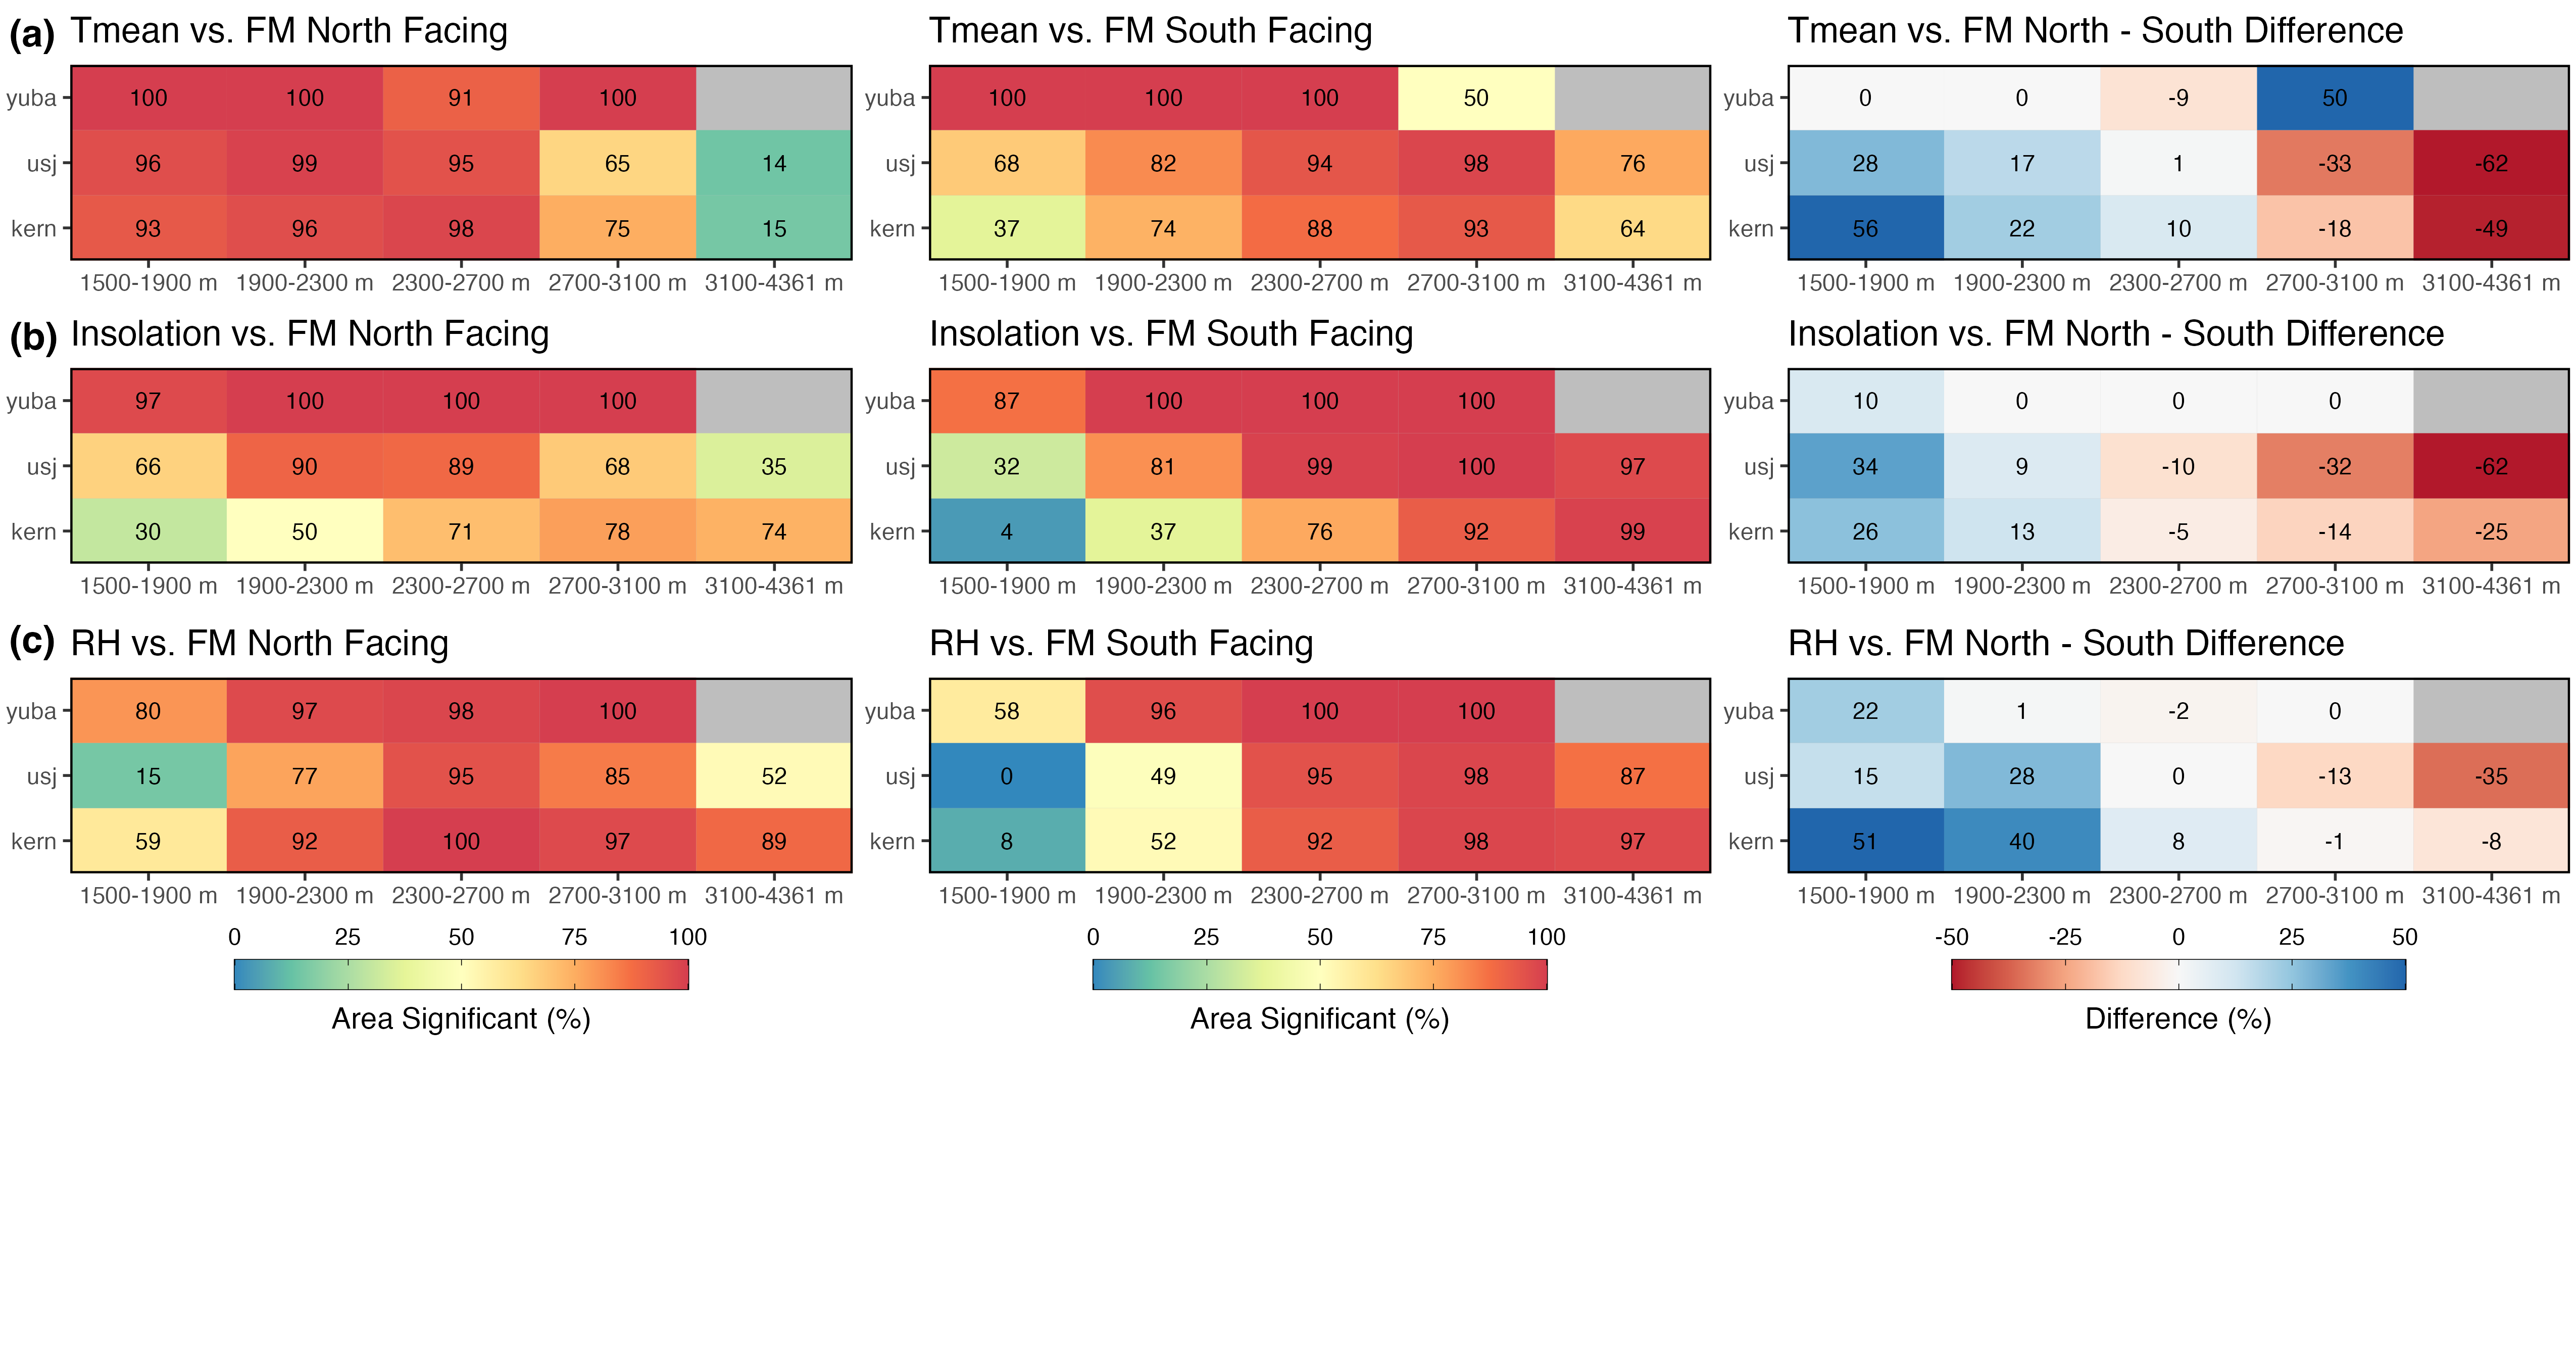
\includegraphics[width=\textwidth]{figures/ch2_figs/metvars_fm_heatmaps_v4.png}
\caption{Heat maps of the displaying percentage of area in each EZ with significant trends (p $< .05$) for \textbf{(a)} T\textsubscript{mean}, \textbf{(b)} RH, \textbf{(c)} insolation for the 32-year study period. The panels are split into north (left), south facing (center) slopes, and the difference between the two (right). The color bars correspond to the values within a given panel.}
\label{fig:met_boxplots}
\end{figure*}

%==============================================================================
%==============================================================================
%==============================================================================
\hypertarget{ch2-discussion}{\section{Discussion}\label{ch2-discussion}}
\hypertarget{ch2-discussion-1}{\section{Key Findings}\label{ch2-discussion-1}}



Our results show substantial differences between all the snow metrics across basins and elevation bands with respect to aspect. These results show the complexity and variability of mountain snowpack even within relatively confined areas and suggest that physiographic relationship play an important roll in the physical mechanisms governing snow ablation and accumulations. However, these factors are both sptatial and temporally variable.

At lower elevations warmer temps increase the rate of snow metamorphism (grain growth), increase temp gradients within snowpack (and snowpack and atm), and further increase rate. (Colbeck, Jennings). 

Larger grain size amplifies the absorption of shorwate (wiscomb and warren, 1980, warren 1980). Midwinter ablation increases the concentration of any light absorbing impurities that may be on the surface (hatchet, gleason, skiles/painter). Hatchet et al. document the increase frequence and length of mid winter dry spells in the sierras. 

It's imporant to note impacts of forest strucutre on the eneryg balance and therefore snowpack dynamics (roth \& nolin). Aspect is a key control on incoming radiation, thus impact the ecohydrlogic composition of the hill slope, and therefore the snowpack energy balance. South facing hillslopes having a higher energy environment, causing a more evaporatioion, less plant available water, and decrease both the type and density of vegetation of SF slopes. Less overlaying vegetation causes more insolation to interacting with the snow surface, and explains why. Whereas northing slopes have dense vegetation, obsturcuting much of the insolation, and therefore shield north facing slopes to significant winter ablation. At the forest gap scale, these same north vs. south gap patterns are also seen (mussleman 2012, webb 2020)


While not specifically paramterized*** in the SNSR, wind transport can substaintally effecst the distrubitoin of snowpack. Depending on the pervailing wind direction (westerly in the sierra), lee facing slopes tend to have 

While south vs. north facing slopes patterns are well-established and visible throughout many mountain ranges accross the globe, our study is the first the quanity the variations in accumulation season snow dynamitcs across various basins in a socioeconomic important mountain region. 

While the course scale of the meteorological data does not capture complex microclimates, previous works suggest that temperatures is warmer on south facing aspects.


-pomeroy (2009) long wave effects on cannopy

The gridMET SRAD data shows both an elevational and latiditunal gradident in values. Our CS insolation model does not account for these variations, and would likely amplify the findings presented herin.

However, the SNSR doesn’t directly address the secondary radiativate forcing, therefore we effect of aspect on snowmelt processes would be amplified.

%==============================================================================
%==============================================================================
%==============================================================================
\hypertarget{ch2-conclusions}{\section{Conclusions}\label{ch2-conclusions}}
hello

\clearpage
\bibliographystyle{apalike}
\setstretch{1}
\bibliography{ch2.bib}
\setstretch{1.5}